%%%%%%%%%%%%%%%%%%%%%%%%%%%%%%%%%%%%%%%%%
% Stylish Article
% LaTeX Template
% Version 2.1 (1/10/15)
%
% This template has been downloaded from:
% http://www.LaTeXTemplates.com
%
% Original author:
% Mathias Legrand (legrand.mathias@gmail.com) 
% With extensive modifications by:
% Vel (vel@latextemplates.com)
%
% License:
% CC BY-NC-SA 3.0 (http://creativecommons.org/licenses/by-nc-sa/3.0/)
%
%%%%%%%%%%%%%%%%%%%%%%%%%%%%%%%%%%%%%%%%%

%----------------------------------------------------------------------------------------
%	PACKAGES AND OTHER DOCUMENT CONFIGURATIONS
%----------------------------------------------------------------------------------------

\documentclass[fleqn,10pt]{SelfArx} % Document font size and equations flushed left

\usepackage[english]{babel} % Specify a different language here - english by default

\usepackage{lipsum} % Required to insert dummy text. To be removed otherwise
\usepackage{graphicx}
\graphicspath{ {./img/} }
\usepackage{float}
\usepackage{hyperref}
%----------------------------------------------------------------------------------------
%	COLUMNS
%----------------------------------------------------------------------------------------

\setlength{\columnsep}{0.55cm} % Distance between the two columns of text
\setlength{\fboxrule}{0.75pt} % Width of the border around the abstract

%----------------------------------------------------------------------------------------
%	COLORS
%----------------------------------------------------------------------------------------

\definecolor{color1}{RGB}{0,0,90} % Color of the article title and sections
\definecolor{color2}{RGB}{0,20,20} % Color of the boxes behind the abstract and headings

%----------------------------------------------------------------------------------------
%	HYPERLINKS
%----------------------------------------------------------------------------------------

\usepackage{hyperref} % Required for hyperlinks
\hypersetup{hidelinks,colorlinks,breaklinks=true,urlcolor=color2,citecolor=color1,linkcolor=color1,bookmarksopen=false,pdftitle={Title},pdfauthor={Author}}

%----------------------------------------------------------------------------------------
%	ARTICLE INFORMATION
%----------------------------------------------------------------------------------------

\JournalInfo{Introduction to Data Analysis  and Mining 2022} % Journal information
\Archive{} % Additional notes (e.g. copyright, DOI, review/research article)

\PaperTitle{Spaceship Titanic, Classification report} % Article title

\Authors{Ashok Kamath and Daeyeop Kim\textsuperscript{1}*} % Authors
\affiliation{\textsuperscript{1}\textit{Computer Science, School of Informatics , Computing and Engineering, Indiana University, Bloomington, IN, USA}} % Author affiliation


\Keywords{Spaceship --- Classification --- Prediction} % Keywords - if you don't want any simply remove all the text between the curly brackets
\newcommand{\keywordname}{Keywords} % Defines the keywords heading name

%----------------------------------------------------------------------------------------
%	ABSTRACT
%----------------------------------------------------------------------------------------

\Abstract{In this report, we attempt to classify passengers on a spaceship as transported or not and utilized the classification models to predict Transported or not based on the classification model}

%----------------------------------------------------------------------------------------

\begin{document}

\flushbottom % Makes all text pages the same height

\maketitle % Print the title and abstract box

\tableofcontents % Print the contents section

\thispagestyle{empty} % Removes page numbering from the first page




%----------------------------------------------------------------------------------------
%Problem and Data Description
%----------------------------------------------------------------------------------------


\section{Problem and Data Description} % The \section*{} command stops section numbering

For the spaceship dataset, the problem is predicting the classification of passengers as to whether they were transported to another dimension. 

There are 14 attributes and 8693 entries in the training set and there are 13 attributes and 4277 entries in the test set. Therefore, the train-test-split ratio is about 2/3 for training and 1/3 for testing. There is one less attribute for the test set because the classification variable is not there. 

There are 6 numerical attributes in the dataset. 5 attributes, Room Service, Food Court, Shopping Mall, Spa and VR Deck, are all monetary measures so they are ratio measurements. These 5 attributes describe how much a passenger spent on the attribute. Age is another ratio variable since it has a true zero point but for this dataset it is discrete. The categorical attributes of the data are the Home Planet, Cryo-Sleep, Cabin, Destination, and VIP features. 

The Home Planet is the planet that the passenger departed from while Cryo Sleep is whether the passenger chose to be put to an extended sleep during the space trip. Cabin is the cabin information for the passenger and is in the form of deck/num/side. Side is either P, which means Port, or S, which means Starboard. 

\bigskip
\bigskip

%----------------------------------------------------------------------------------------
%	Data Preprocessing $\&$ Exploratory Data Analysis
%----------------------------------------------------------------------------------------

\section{Data Preprocessing $\&$ Exploratory Data Analysis} % The \section*{} command stops section numbering

\subsection{Handling Missing Values}
For handling the missing values, we first found the number of missing values for each attribute. Most of the columns had missing values. From there, for the ratio attributes, we looked at the distribution and found that for all the monetary attributes (Room Service, Food Court, Shopping Mall, Spa and VR Deck), a majority of the values were 0 since the median was 0. For that reason, we decided to fill in the missing values for these columns with 0. For Age, on the other hand, the median and the mean were similar so we chose the mean to fill in the missing values. For the categorical attributes of Home Planet and Destination, we found the mode and then filled in the missing values with this figure since there was no average or median because it is categorical data.

\begin{figure}[H]
    \centering
    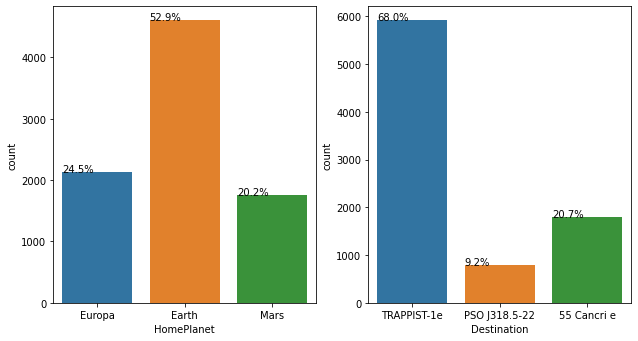
\includegraphics[width=7cm,height=3cm]{img/output.png}
    \caption{Home Planet and Destination Before covering missing value}
    \label{fig:my_label}
    \centering
    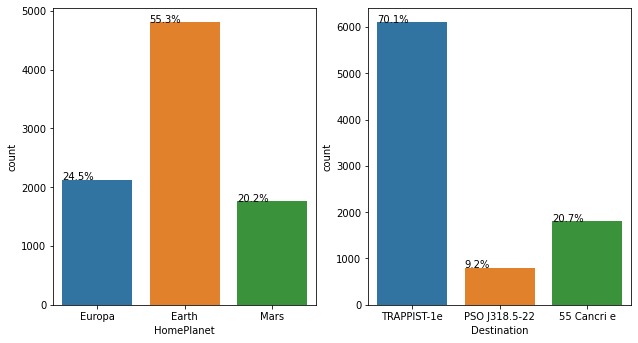
\includegraphics[width=7cm,height=3cm]{img/spaceshiptwithplanetanddestination.png}
    \caption{Home Planet and Destination After covering missing value}
    \label{fig:my_label}
\end{figure}
As this count-plots shows that there were percentages change after the missing value covers. Like Figure1 and 2, there were 1 or less percentage were changed so it does not effect to the result at all. 

\subsection{Exploratory Data Analysis}
Before the we check for the classifications and do all the technique for this problem.
We checked the target variable is balanced or not.
\begin{figure}[H]
    \centering
    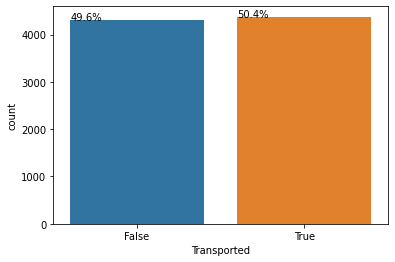
\includegraphics[width=7cm, height=6cm]{img/transported.png}
    \caption{Graph for Target variable("Transported")}
    \label{fig:my_label}
\end{figure}    
From the count plot, we can see that the target variable is 49.5\% False and 50.4\% True. We can see that the target variable is highly balanced so we don't have to consider technique for under or over sampling. 
\begin{figure}[H]
    \centering
    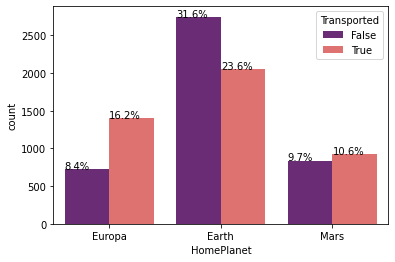
\includegraphics[width=7cm, height=6cm]{img/homeplanet.png}
    \caption{Graph for HomePlanet with Target("Transported")}
    \label{fig:my_label}
\end{figure} 
To better understand the data, we started by creating some count plots. Our count plot of Home Planet, which was grouped by whether the passenger was transported, showed that about 2/3 of those from Europa were transported. For the passengers that were from Earth, they had around a 60 \% chance of not being transported. For Mars, however, it was evenly distributed.
\begin{figure}[H]
    \centering
    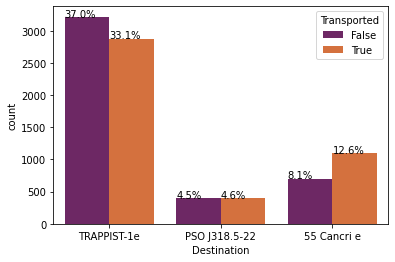
\includegraphics[width=7cm, height=6cm]{img/destination.png}
    \caption{Graph for Destination with Target("Transported")}
    \label{fig:my_label}
\end{figure}
For the Destination attribute, if the passenger was headed for TRAPPIST-1e or PSOJ318.5-22, there was not much of a difference in whether the passenger was transported, but if the passenger was heading towards 55 Cancri-e, then they had about a 60 \% chance of being transported. 
\begin{figure}[H]
    \centering
    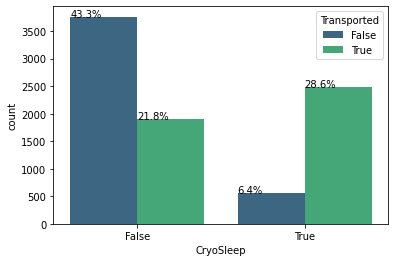
\includegraphics[width=8cm, height=6cm]{img/crysleepaftermissingcover.png}
    \caption{Graph for CyroSleep with Target("Transported")}
    \label{fig:my_label}
\end{figure}    
For the CryoSleep attribute, if it was true that the passenger was in this state, then they had an 82\% chance of being transported. If there were not in CryoSleep, then they had a 33\% chance of being transported. This indicates that CryoSleep will be an important variable in predicting the classification of passengers in the test set as to whether they were transported. 
\begin{figure}[H]
    \centering
    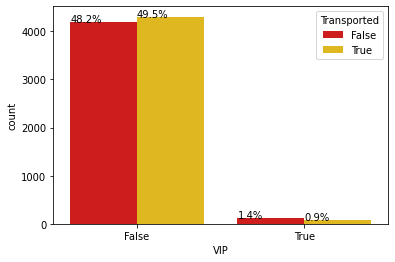
\includegraphics[width=8cm, height=6cm]{img/vip.png}
    \caption{Graph for VIP with Target("Transported")}
    \label{fig:my_label}
\end{figure}  
For the VIP attribute, we found that the distribution for transportation was quite even if the passenger was not VIP. If the passenger was VIP, on the other hand, then there was only a 40\% chance of being transported, which means that this variable is helpful in predicting transportation only for the passengers who are VIP.
\begin{figure}[H]
    \centering
    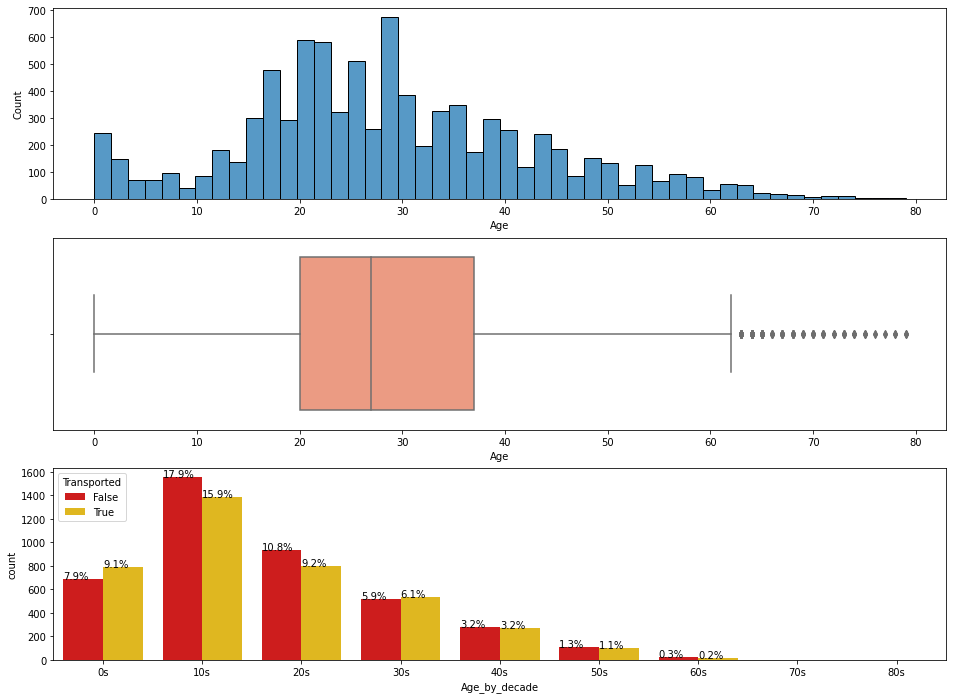
\includegraphics[width=7cm, height=6cm]{img/spaceshipwithagedistribution.png}
    \caption{Graph for Age distribution and Age with Target("Transported")}
    \label{fig:my_label}
\end{figure}  
For the Age attribute, distribution shows that 15~ 30years old were most number of groups in the ship and over 65 years old were least number of groups in the ship And count-plot shows 10s, 20s has higher percentage to be not transported than transported. 0s, 30s has higher percentage to be transported than not transported. Also, over 30s has about equal or 0.1\% different percentage transported and not transported. 

\begin{figure}[H]
    \centering
    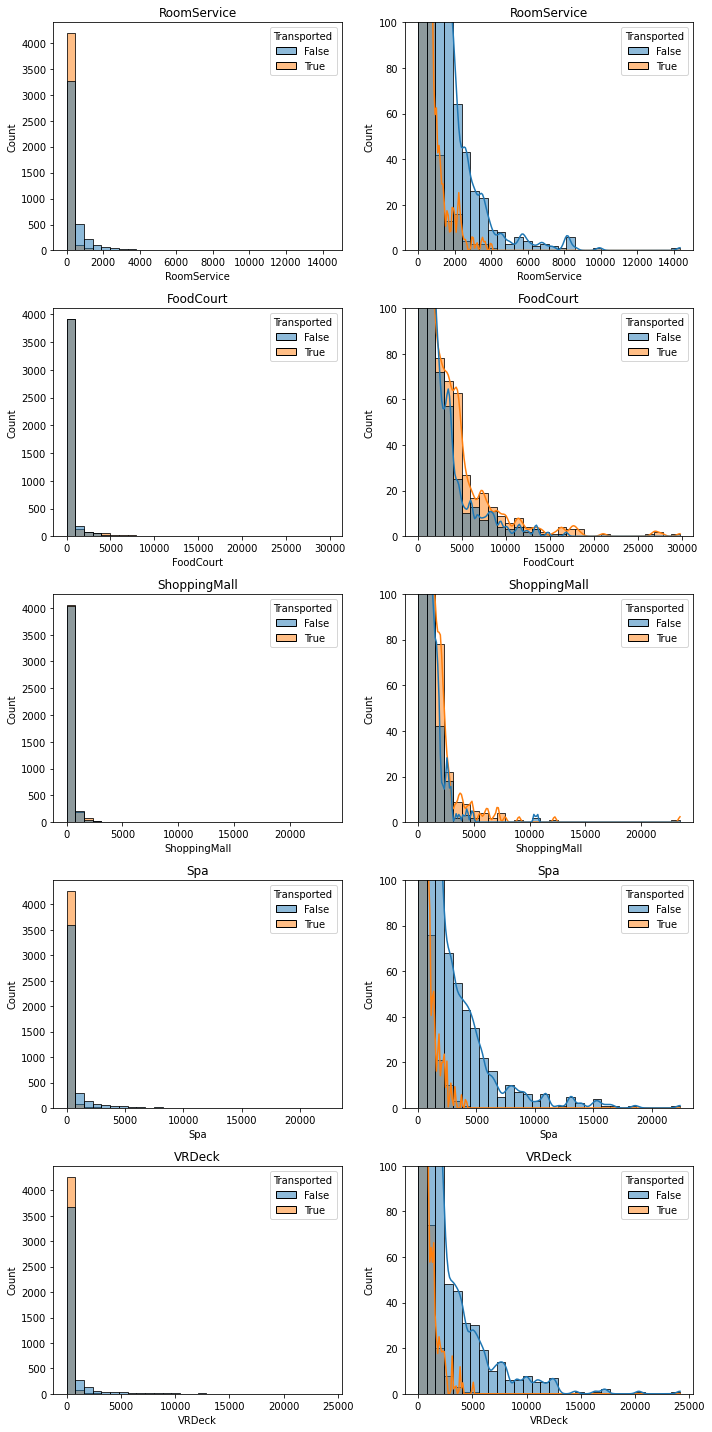
\includegraphics[width=7cm, height=10cm]{img/numeric.png}
    \caption{Graph for Bill amounts with Target("Transported")}
    \label{fig:my_label}
\end{figure}  
For the numeric categories(Room service, Food Court, Shopping Mall, Spa, VR Deck) attribute, the graphs are shows that there are small number of outliers and people who were transported tended to spend less.The left-side graph show mostly which means the most people did not spend any money. And the right-side graphs show on right graphs, the distribution of spending decays exponentially. Since Room Service, Spa, and VR Deck have different distribution to Food court, and Shopping mall, we can might think of think as luxury and essential amenities.

We did PCA since it gives a low dimensional representation of the data while it preserves the local and global structure. We conducted the principal component analysis (the number of principal components is designated as 3). Also, for PCA, we reduced dimension to an array of size (8693, 13). We used the 'extended variance ratio' method to obtain the variance ratio (unique value/total eigenvalue) and it describes variance which represents the information described using specific principal components.
\begin{figure}[H]
    \centering
    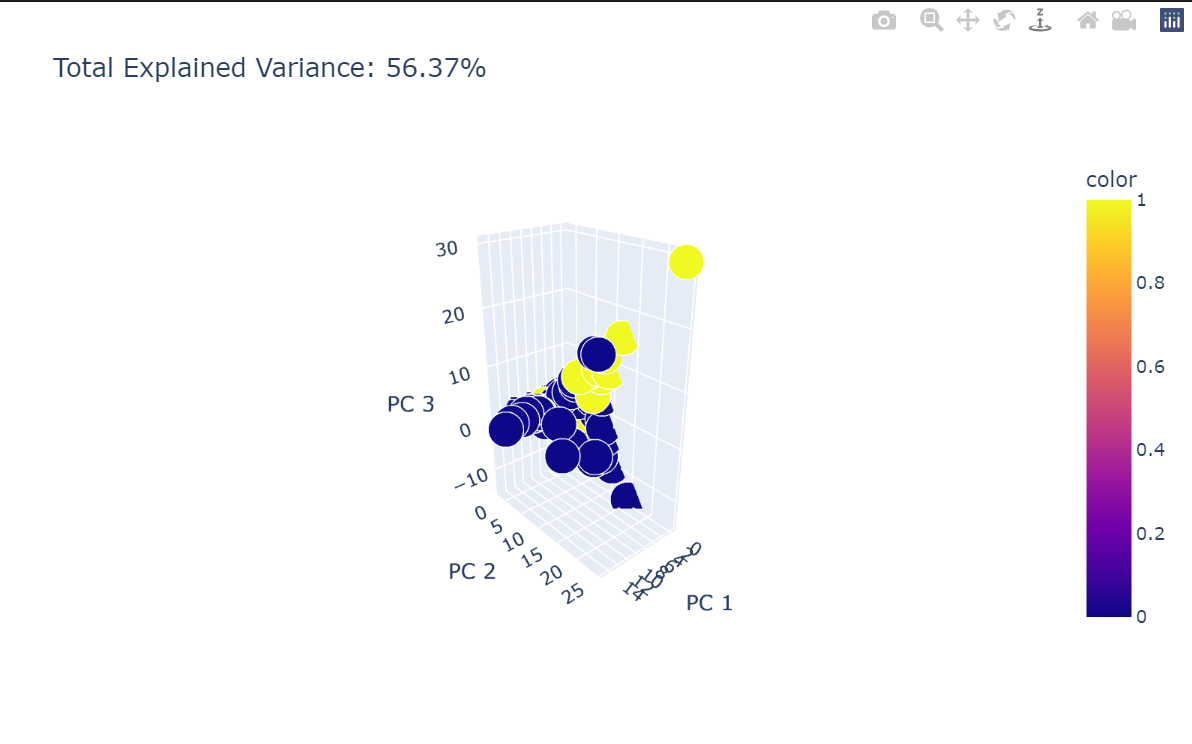
\includegraphics[width=7cm, height=8cm]{img/pca.png}
    \caption{Visualize the distribution of principal component in 3-Dimension}
    \label{fig:my_label}
\end{figure}
As this 3-Dimension scatter plot show, it explains 56.37\% of the principle component from the original data. 
\begin{figure}[H]
    \centering
    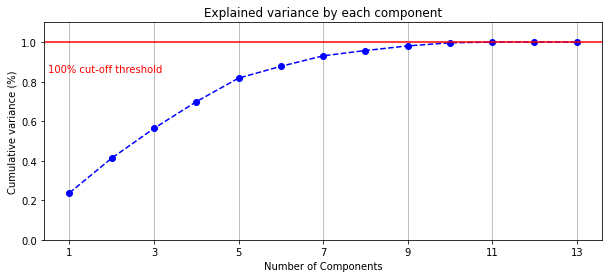
\includegraphics[width=7cm, height=6cm]{img/PCA2.png}
    \caption{Graph for explained variance by each component)}
    \label{fig:my_label}
\end{figure}
As this graphs shows, More than 6 principle component describe the most of distribution.

\bigskip
\bigskip

%----------------------------------------------------------------------------------------
 % Algorithm and Methodology
%----------------------------------------------------------------------------------------


\section{Algorithm and Methodology}

For this classification problem, the first method we used was the k-nearest neighbors method. It works by taking an entry that we want to classify, computing the distance between this point and all the points in the training data, and then using the majority class of the nearest neighbors within the training data to classify the testing point. The k-nearest neighbors method is a lazy learner but it can be very powerful when used in the right situations. 

Another technique we chose was logistic regression since it can predict a binary outcome, such as transported or not. This supervised machine learning algorithm executes the classification by using the logistic function along with maximum likelihood estimation. Besides k-nearest neighbors and logistic regression, we also used the Naive Bayes classifier, which uses Bayes’ Theorem and prior probabilities to arrive at a posterior probability for Transported and Not Transported. 

Additionally, we created a decision tree classifier, which cycles through the attributes to see which can best reduce the entropy of the data and then uses that attribute as a decision node in the tree. It can use a variety of measures to see how much the entropy decreases, ranging from information entropy to Gini Impurity. A more advanced model similar to the decision is the random forest model, which is an ensemble method that uses a multitude of decision trees and then takes the majority vote of the decision trees to classify a data point. A random forest model uses bootstrapping to create the decision trees and then randomly selects attributes to use for each decision tree. 

Another model we used for this classification problem was extreme gradient boosting. This technique is similar to the random forest model since they are both ensemble methods composed of decision trees. The difference, however, is how the decision trees are constructed. While random forest uses bootstrapping, extreme gradient boosting uses gradient descent on the error residuals of the previously created decision tree to create the next decision tree. We wanted to try this algorithm since it has been very popular over the last few years in the data science community. 

We also used the Light Gradient Boosting Machine, which is a distributed, fast decision tree model. Not to mention, we also experimented with the Gradient Boost machine learning algorithm, which is similar to the Extreme Gradient Boosting model and the Light Gradient Boosting Machine. Lastly, we used a neural network multi-layer perceptron as our final model, which uses gradient descent over multiple levels of weighted nodes to arrive at a prediction for the class. 

\bigskip
\bigskip
%----------------------------------------------------------------------------------------
 % Experiments and Results
%----------------------------------------------------------------------------------------
\section{Experiments and Results}
First, we checked the correlation matrix to find the relationship between all the features while also checking for redundancy. 
\begin{figure}[H]
    \centering
    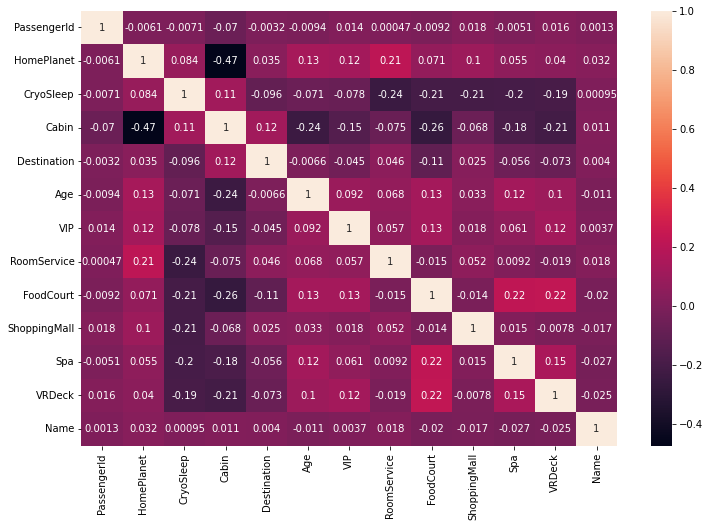
\includegraphics[width=7cm, height=6cm]{img/ssss.png}
    \caption{Graph for explained variance by each component)}
    \label{fig:my_label}
\end{figure}
 The correlation matrix shows that Passenger Id, Cabin, Age, Name can be selected for drop.

\bigskip

\begin{tabular}{ |p{3cm}|p{3cm}|  }
\hline
\multicolumn{2}{|c|}{Accuracy percentage before K-fold} \\
\hline
Model Name& Accuracy percentage \\
\hline
LGBM & 78.29\% \\
XGB & 78.29\%\\
Random forest & 78.75\% \\
Gradient Boost    & 78.33\% \\
Logistic Regression & 78.20\%\\
NNMLP & 77.28\% \\
KNN & 73.55\%  \\
Decision Tree & 74.06\% \\
Naive Bayes	 & 68.54\%  \\
\hline
\end{tabular}

\begin{tabular}{ |p{3cm}|p{3cm}|  }
\hline
\multicolumn{2}{|c|}{Accuracy percentage after K-fold} \\
\hline
Model Name& Accuracy percentage \\
\hline
LGBM & 79.32\% \\
XGB & 78.91\%\\
Random forest & 78.89\% \\
Gradient Boost    & 78.89\% \\
Logistic Regression & 78.68\%\\
NNMLP & 77.37\% \\
KNN & 76.10\%  \\
Decision Tree & 75.00\% \\
Naive Bayes	 & 69.60\%  \\
\hline
\end{tabular}

For k-nearest neighbors, the cross validation accuracy on the training data was about 76.10\%. We expected to see a mediocre rate of accuracy for this method since a lazy learner may not work that well on this type of data. 

For logistic regression, on the other hand, the cross validation accuracy on the training data was about 78.68\%, which was a major improvement from the k-nn accuracy rate. Logistic regression is a powerful tool for binary classification, justifying the result. 

In contrast, Naive Bayes performed weakly for cross validation accuracy on the training data, which could be expected since Naive Bayes makes an assumption of independence among all the features, yet it was highly unlikely that features such as RoomService, FoodCourt and ShoppingMall were independent. If someone spends a lot at one location, then they are likely to spend a lot at another location, which implies dependence. 

The decision tree performed better for cross validation accuracy on the training data than k-nn and Naive Bayes, but was not as accurate as logistic regression. The decision tree had an accuracy of about 75.00\%. We were surprised to see the decision tree perform better than k-nn and Naive Bayes since decision trees can sometimes have trouble with accuracy due to overfitting. With the right parameters, however, such as maximum depth, that problem can be avoided. 

From there, our ensemble methods had higher accuracy rates for cross validation on the training data. The random forest classifier had performed at about 79.32\% while the extreme gradient boosting model had an accuracy rate of about 78.91\%. The Light Gradient Boosting Machine and the Gradient Booster Classifier had accuracies around 78.89\% too. The Neural Network multi-layer perceptron performed at an accuracy of about 77.37\%, but took a long time to train.

\begin{figure}[H]
    \centering
    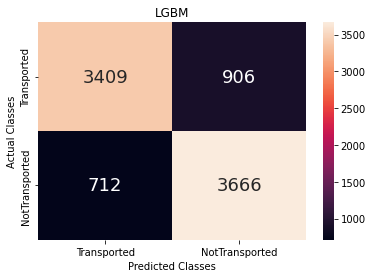
\includegraphics[width=7cm, height=6cm]{img/confusionmatrix.png}
    \caption{confusion matrix for LGBM (most accurate model)}
    \label{fig:my_label}
\end{figure}
Since the confusion matrix is a table for comparing predicted and actual values to measure prediction performance through training we can find the accuracy in the diagonal of confusion matrix, precision in the horizontal of confusion matrix, and recall in the vertical part of confusion matrix.
\bigskip

\begin{tabular}{ |p{1.18cm}|p{1.6cm}|p{2.1cm}|p{1.2cm}|}
\hline
\multicolumn{4}{|c|}{classification report} \\
\hline
rates & Transported & NotTransported & accuracy\\
\hline
precision & 0.827226 &0.801837 & 0.813873  \\
recall & 0.790035	 & 0.837369&0.813873\\
f1-score & 0.808203&  0.819218 &	0.813873 \\
\hline
\end{tabular}
\bigskip

According to our model, we get a precision accuracy of about 81.40\% and a recall accuracy of about 81.40\%. For f1-score, we do not need to use this since the target variable is balanced.

Since the Light Gradient Boosting Machine worked the best in cross validation, we used that model on the test data for predictions. This gave us an accuracy rate of 79.32\%, which placed us on the leader board at a rank of 1118 out of 1866 teams. 

\bigskip
\bigskip

%----------------------------------------------------------------------------------------
 % Summary and Conclusions
%----------------------------------------------------------------------------------------
\section{Summary and Conclusions}
For this section, the objective was to classify passengers as transported or not. The training set had more than 8500 entries while the test set had about 4300. There were 13 attributes, excluding the attribute of transported or not. Many of the attributes measured how much a passenger spent at different locations on the spaceship titanic. 

When handling missing values, we evaluated whether an attribute’s missing values would best be filled by the median, mean or mode of the attribute based on the distribution of the attribute. Through our exploratory data analysis, we found important pieces of information. We discovered that ⅔ of those from Europa were transported and if a passenger was in CryoSleep, then they had an 82\% chance of being transported. If they were not in CryoSleep, then they had only a 33\% chance of being transported. We also noticed that the passengers who were VIP had only a 40\% chance of being transported while there was not much distinction among those who were not VIP. 

When modeling for this problem, we used a variety of algorithms, ranging from k-nearest neighbors, Naive Bayes and Decision Tree to Extreme Gradient Boosting and Random Forest. Ultimately, the Light Gradient Boosting Machine Classifier was the most accurate for cross validation on the training data so we used that on the test data and for the Kaggle submission, which resulted in an accuracy rate of 78.98\%, placing us on the leaderboard at a rank of 1118 out of 1866 teams. The best submission, in rank 1, had a score of about 82\%. Our result could be improved by hyper-tuning the model, which could be done through a grid search. 


\bigskip
\bigskip
\bigskip    



%----------------------------------------------------------------------------------------
%	REFERENCE LIST
%----------------------------------------------------------------------------------------

\bibliographystyle{unsrt}

\bibliography{sample}
\href{https://www.kaggle.com/code/samuelcortinhas/spaceship-titanic-a-complete-guide#Libraries}{SAMUEL CORTINHAS /Spaceship Titanic: A complete guide}
%----------------------------------------------------------------------------------------

\end{document}